\section{Introduction}
%\input{figure_teaser}
%In this paper we focus
%on the task of detecting and estimating poses of multiple people in
%uncontrolled real-world images.
Human body pose estimation methods have become
increasingly reliable.
% in localizing body joints.
Powerful body part
detectors \cite{Tompson:2015:EOL} in combination with
tree-structured body models \cite{tompson14nips,chen14nips} show
impressive results on diverse datasets
\cite{johnson11cvpr,andriluka14cvpr,sapp13cvpr}.
% \pgsuggestinstead{.
  These benchmarks promote pose estimation of
  single pre-localized persons but exclude
  scenes with multiple people.
%}{where people are pre-localized and it
%is required to estimate the pose of one person only. However these
%benchmarks specifically exclude scenes with multiple people that
%might overlap each other (\eg.~ as in Fig.~\ref{fig:teaserfig})}.
%\pgsuggest{
%
  This problem definition has been a driver for % the development of
  progress, but also falls short on representing a
  realistic sample of real-world images. Many photographs contain multiple
  people of interest (see Fig~\ref{fig:overview})
  and it is unclear whether single pose
  approaches generalize directly. We argue that
  the multi person case deserves more attention since it is an important real-world task.
  % that is of interest
  %for users and different applications.
  % shows samples of the MPII dataset~\cite{andriluka14cvpr}.

\tabcolsep 1.5pt
\begin{figure}
  \centering
  \begin{tabular}{c c c }
%%   \includegraphics[width=0.31\linewidth]{figures/teaser/imgidx_0156_init_graph.pdf}&
%%   \includegraphics[width=0.31\linewidth]{figures/teaser/imgidx_0156_graph.pdf}&
%%   \includegraphics[width=0.31\linewidth]{figures/teaser/imgidx_0156_sticks.pdf}
%%   \\
  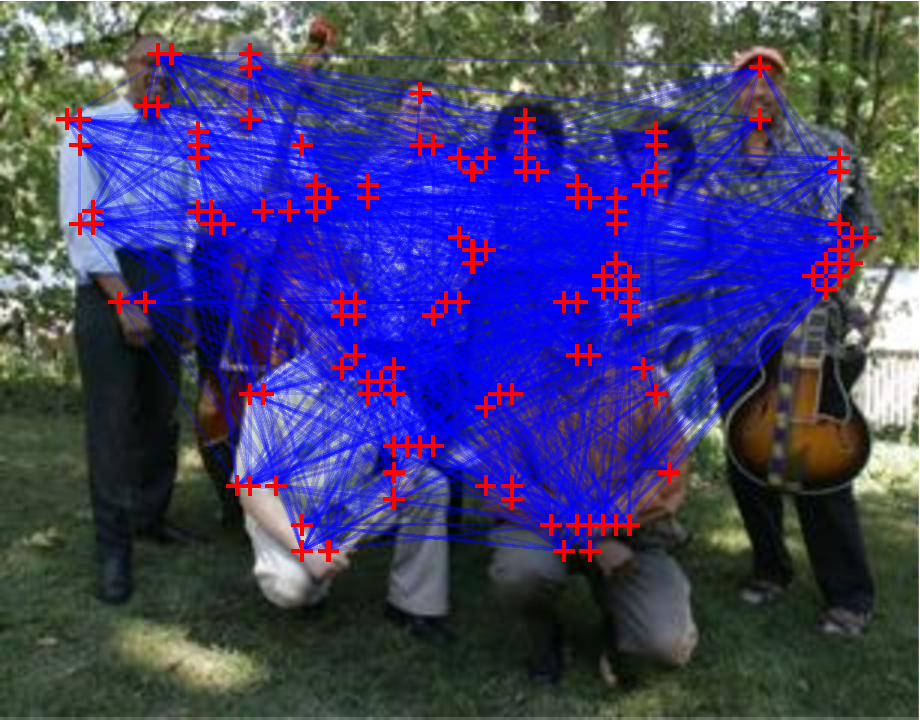
\includegraphics[width=0.31\linewidth]{imgidx_0063_init_graph.pdf}&
  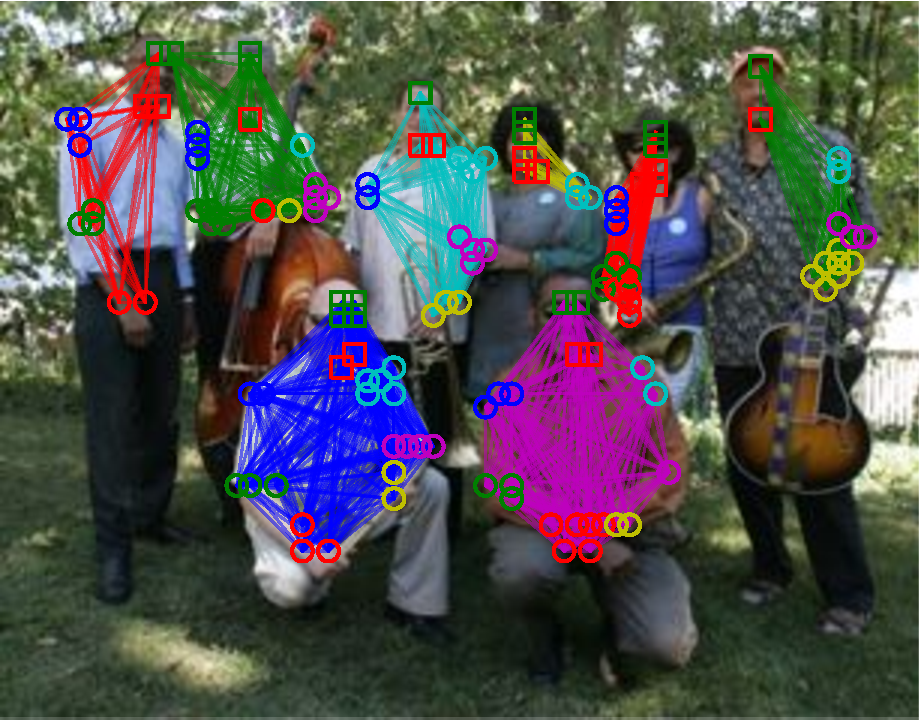
\includegraphics[width=0.31\linewidth]{imgidx_0063_graph.pdf}&
  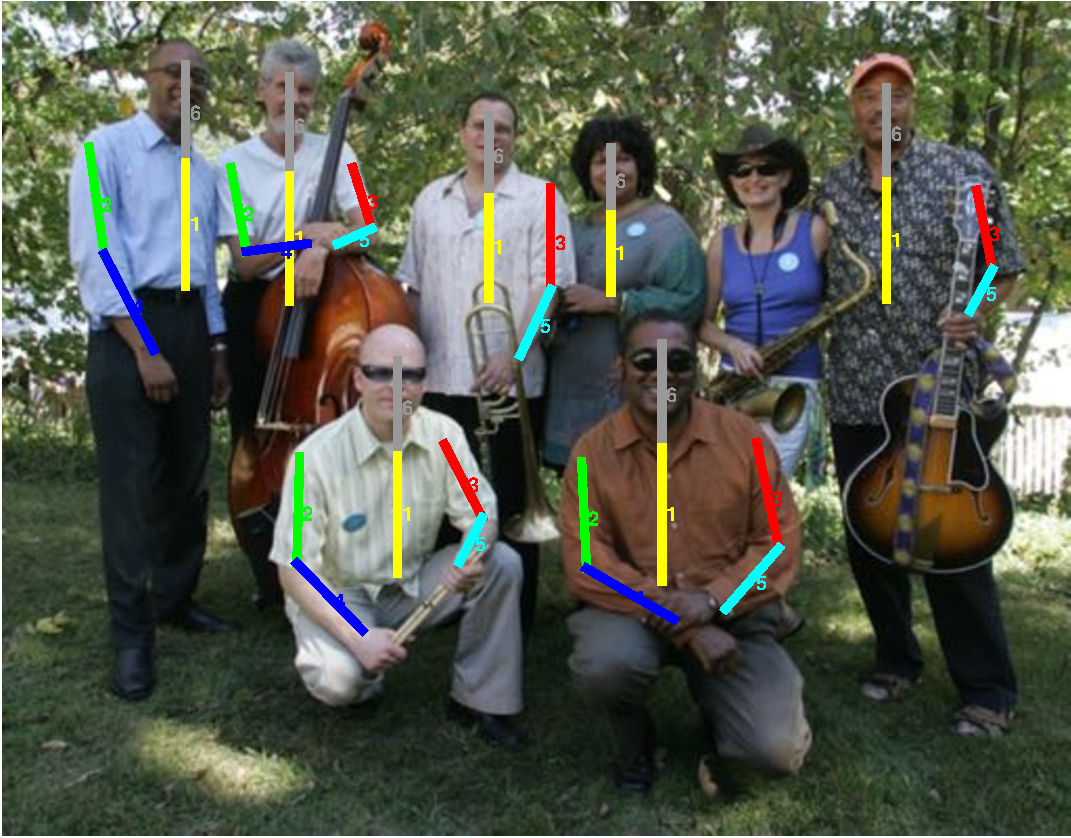
\includegraphics[width=0.31\linewidth]{imgidx_0063_sticks.pdf}
  \\
  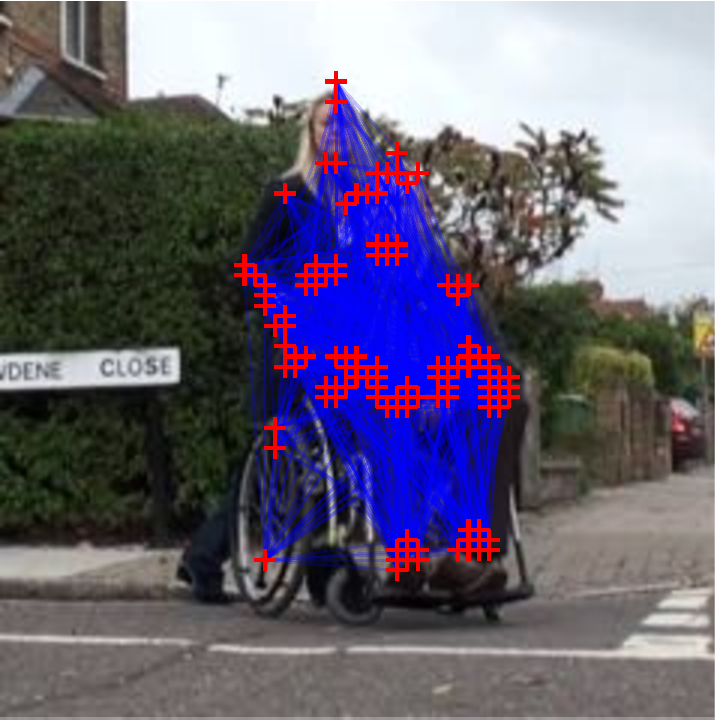
\includegraphics[width=0.31\linewidth]{imgidx_0672_init_graph.pdf}&
  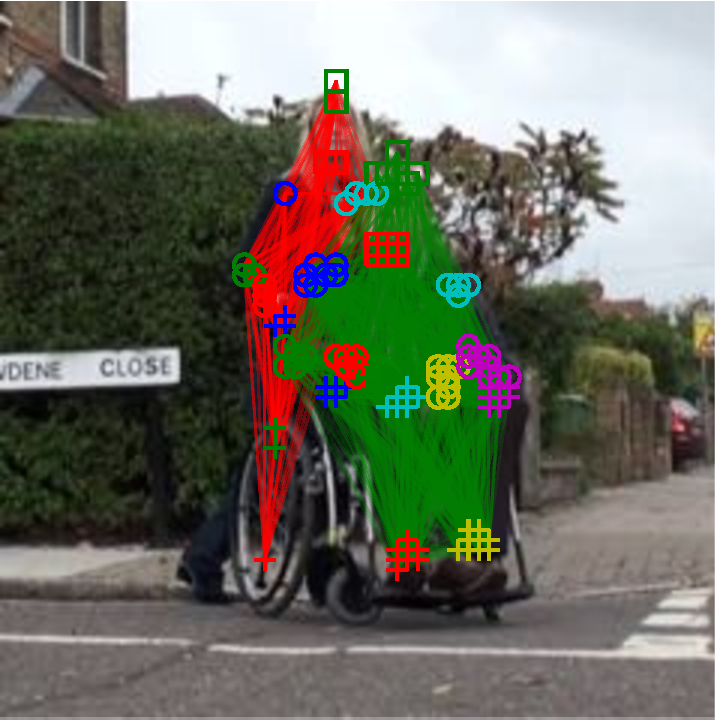
\includegraphics[width=0.31\linewidth]{imgidx_0672_graph.pdf}&
  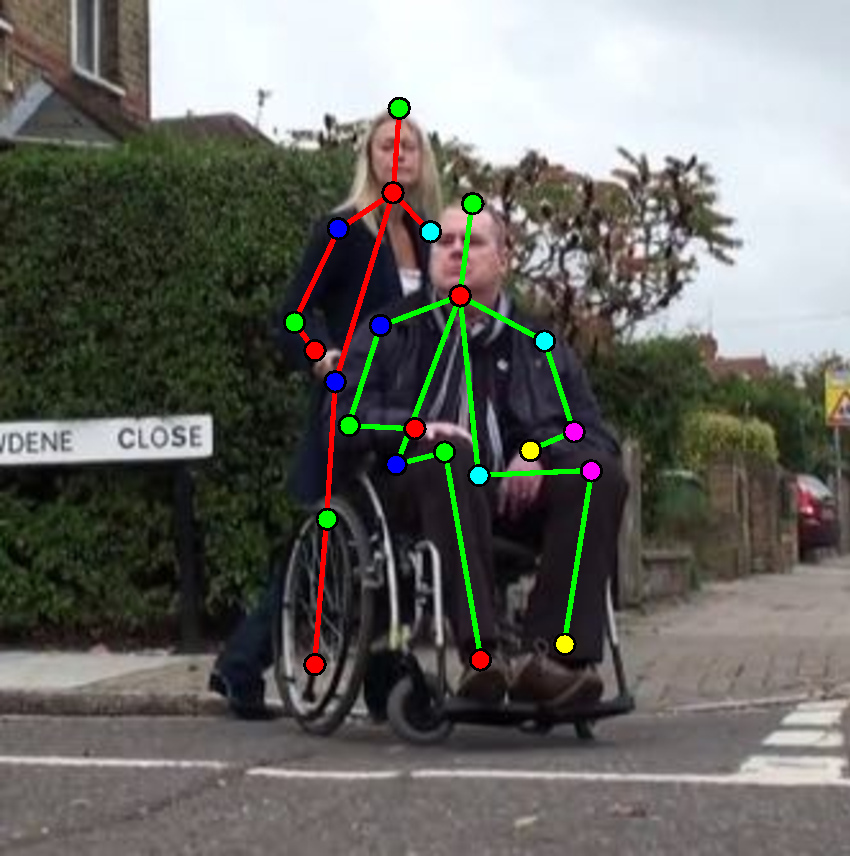
\includegraphics[width=0.31\linewidth]{imgidx_0672_sticks.pdf} 
  \\
  %[2 30 32 45 60 63 66 69 74 78 80 83 89 114 146 156 161 169]
%% %%   \includegraphics[width=0.31\linewidth]{figures/teaser/imgidx_0002_init_graph.pdf}&
%% %%   \includegraphics[width=0.31\linewidth]{figures/teaser/imgidx_0002_graph.pdf}&
%% %%   \includegraphics[width=0.31\linewidth]{figures/teaser/imgidx_0002_sticks.pdf}
%% %%   \\

%%   \includegraphics[width=0.31\linewidth]{figures/teaser/imgidx_0030_init_graph.pdf}&
%%   \includegraphics[width=0.31\linewidth]{figures/teaser/imgidx_0030_graph.pdf}&
%%   \includegraphics[width=0.31\linewidth]{figures/teaser/imgidx_0030_sticks.pdf}
%%   \\
%%   \includegraphics[width=0.31\linewidth]{figures/teaser/imgidx_0032_init_graph.pdf}&
%%   \includegraphics[width=0.31\linewidth]{figures/teaser/imgidx_0032_graph.pdf}&
%%   \includegraphics[width=0.31\linewidth]{figures/teaser/imgidx_0032_sticks.pdf}
%%   \\
%%   \includegraphics[width=0.31\linewidth]{figures/teaser/imgidx_0045_init_graph.pdf}&
%%   \includegraphics[width=0.31\linewidth]{figures/teaser/imgidx_0045_graph.pdf}&
%%   \includegraphics[width=0.31\linewidth]{figures/teaser/imgidx_0045_sticks.pdf}
%%   \\
%%   \includegraphics[width=0.31\linewidth]{figures/teaser/imgidx_0066_init_graph.pdf}&
%%   \includegraphics[width=0.31\linewidth]{figures/teaser/imgidx_0066_graph.pdf}&
%%   \includegraphics[width=0.31\linewidth]{figures/teaser/imgidx_0066_sticks.pdf}
%%   \\

%% %%   \includegraphics[width=0.31\linewidth]{figures/teaser/imgidx_0069_init_graph.pdf}&
%% %%   \includegraphics[width=0.31\linewidth]{figures/teaser/imgidx_0069_graph.pdf}&
%% %%   \includegraphics[width=0.31\linewidth]{figures/teaser/imgidx_0069_sticks.pdf}
%% %%   \\
%% %%   \includegraphics[width=0.31\linewidth]{figures/teaser/imgidx_0074_init_graph.pdf}&
%% %%   \includegraphics[width=0.31\linewidth]{figures/teaser/imgidx_0074_graph.pdf}&
%% %%   \includegraphics[width=0.31\linewidth]{figures/teaser/imgidx_0074_sticks.pdf}
%% %%   \\
%% %%   \includegraphics[width=0.31\linewidth]{figures/teaser/imgidx_0080_init_graph.pdf}&
%% %%   \includegraphics[width=0.31\linewidth]{figures/teaser/imgidx_0080_graph.pdf}&
%% %%   \includegraphics[width=0.31\linewidth]{figures/teaser/imgidx_0080_sticks.pdf}
%% %%   \\

%%   \includegraphics[width=0.31\linewidth]{figures/teaser/imgidx_0083_init_graph.pdf}&
%%   \includegraphics[width=0.31\linewidth]{figures/teaser/imgidx_0083_graph.pdf}&
%%   \includegraphics[width=0.31\linewidth]{figures/teaser/imgidx_0083_sticks.pdf}
%%   \\
  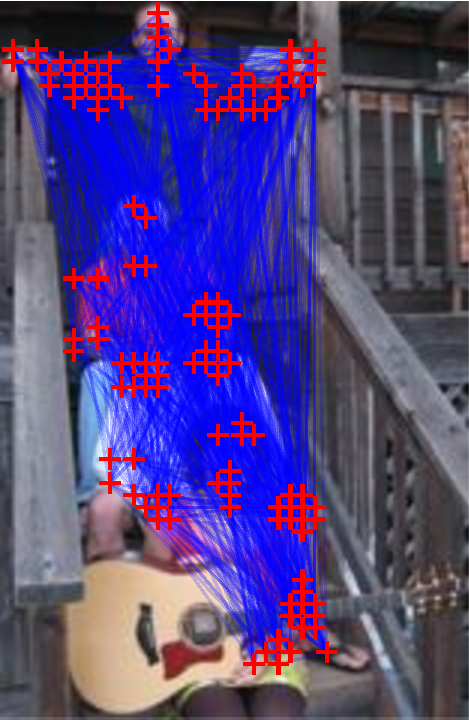
\includegraphics[width=0.31\linewidth]{imgidx_0089_init_graph.pdf}&
  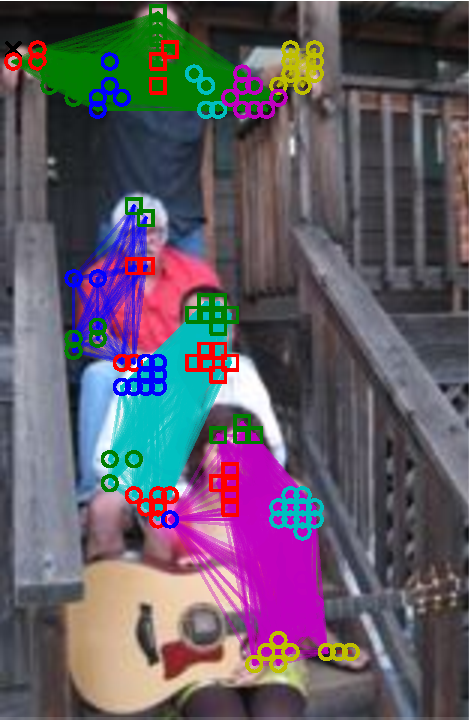
\includegraphics[width=0.31\linewidth]{imgidx_0089_graph.pdf}&
  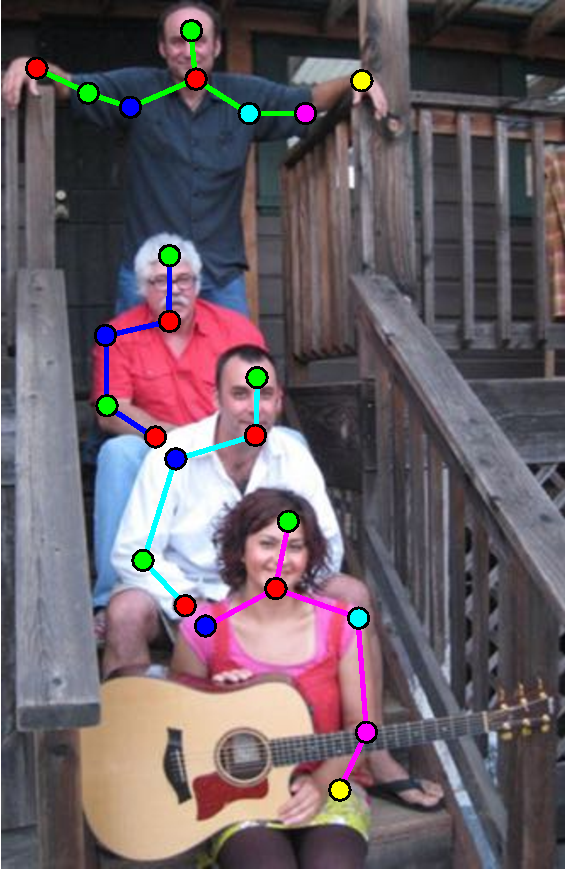
\includegraphics[width=0.31\linewidth]{imgidx_0089_sticks.pdf}
  \\
%%   \includegraphics[width=0.31\linewidth]{figures/teaser/imgidx_0114_init_graph.pdf}&
%%   \includegraphics[width=0.31\linewidth]{figures/teaser/imgidx_0114_graph.pdf}&
%%   \includegraphics[width=0.31\linewidth]{figures/teaser/imgidx_0114_sticks.pdf}
%%   \\

%% %%   \includegraphics[width=0.31\linewidth]{figures/teaser/imgidx_0146_init_graph.pdf}&
%% %%   \includegraphics[width=0.31\linewidth]{figures/teaser/imgidx_0146_graph.pdf}&
%% %%   \includegraphics[width=0.31\linewidth]{figures/teaser/imgidx_0146_sticks.pdf}
%% %%   \\
%%   \includegraphics[width=0.31\linewidth]{figures/teaser/imgidx_0161_init_graph.pdf}&
%%   \includegraphics[width=0.31\linewidth]{figures/teaser/imgidx_0161_graph.pdf}&
%%   \includegraphics[width=0.31\linewidth]{figures/teaser/imgidx_0161_sticks.pdf}
%%   \\
%%   \includegraphics[width=0.31\linewidth]{figures/teaser/imgidx_0169_init_graph.pdf}&
%%   \includegraphics[width=0.31\linewidth]{figures/teaser/imgidx_0169_graph.pdf}&
%%   \includegraphics[width=0.31\linewidth]{figures/teaser/imgidx_0169_sticks.pdf}
%%   \\
  (a) & (b) & (c) \\   
  \end{tabular} 

  \caption{Method overview: (a) initial detections (= part
  candidates) and pairwise terms (graph) 
  between all detections that (b) are jointly clustered belonging to
  one person (one colored subgraph = one person) and each part is labeled
  corresponding to its part class (different colors and symbols
  correspond to different body parts); (c) shows the predicted pose
  sticks.}
 \vspace{-1.0em}
  \label{fig:overview}
\end{figure}


  Key challenges inherent to multi person pose estimation are the partial visibility
  of some people,
  %either due to truncation
  %or partial occlusion, and further,
  significant overlap of bounding box regions of people,
%
%In such conditions the number of
%body parts that can be predicted based on the image varies from person
%to person.
%\pgcomment{I do not understand that last sentence}
  and the a-priori unknown number of people in an image.
  The problem thus is to infer the number of persons, assign part detections
  to person instances while respecting geometric and
  appearance constraints.
%}{Since the number
%  of people in the image is not known in advance, this creates a
%  challenging problem where part detections need to be uniquely
%  assigned to unknown number of person instances while respecting
% geometric and appearance constraints.}
  Most strategies use a two-stage inference process
  \cite{pishchulin12cvpr,Gkioxari:2014:UKP,Sun:2011:APM} to first
  detect and then independently estimate poses. This is
  unsuited for cases when people are in close proximity since they
  permit simultaneous assignment of the same body-part candidates to
  multiple people hypotheses.
  %Therefore, in this paper, we approach
  %the pose estimation problem by jointly estimating the number of
  %people in the image, infer their spatial arrangement and reason
  %about body part visibility.

  As a principled solution for multi person pose estimation a model is
  proposed that jointly estimates poses of all people present in an
  image by minimizing a joint objective.  The formulation is based on
  partitioning and labeling an initial pool of body part candidates
  into subsets that correspond to sets of mutually consistent
  body-part candidates and abide to mutual consistency and exclusion
  constraints. The proposed method has a number of appealing
  properties. (1) The formulation is able to deal with an unknown
  number of people, and also infers this number by linking part
  hypotheses. (2) The formulation allows to either deactivate or merge
  part hypotheses in the initial set of part candidates hence
  effectively performing non-maximum suppression (NMS). In contrast to
  NMS performed on individual part candidates, the model incorporates
  evidence from all other parts making the process more reliable.  (3)
  The problem is cast in the form of an Integer Linear Program
  (ILP). Although the problem is NP-hard, the ILP formulation
  facilitates the computation of bounds and feasible solutions with a
  certified optimality gap.

%% Although this problem is NP-hard, the bound
%%   obtained from its dual allows to trade off run-time with a certified optimality gap.
%   { \textcolor{red}{(3) Our
%   approach is an integer linear program, the use
%   of robust optimization techniques allows for guarantees
%   of the optimality of the result with a relative optimality gap below 1\%.}}
% \pgcomment{This (3) is a weak statement. You are
%     basically suggesting that usually there is no sound mathematical
%     foundation.}

% We rely on recent advances in object detection and use CNN-based detector of \cite{} to generate
% initial set of body-part candidates.

% - infer number of people as number of clusters
% - infer visibility / turn off candidates inconsistent with the rest
% - can merge multiple candidates for the same part (NMS), NMS is done while taking info from other
% parts into account (in contrast to standard NMS that would only consider detection score)
% - based on sound mathematical framework, optimization is well understood, can be globally optimized
% (approximate solutions such as Kernighan-Lin available and can be used to speed up inference further \cite{}), other methods that propose global objective require greedy/iterative
% optimization /cite{Ladicky}


% The formulation includes a mechanism of either merging together similar candidates or ignoring
% candidates that are inconsistent with the final solution, thus implicitly performing a non-maximum
% suppression on body-part hypothesis set.

  This paper makes the following contributions. The main
  contribution is the derivation of a joint detection and pose estimation
  formulation cast as an integer linear program.
  Further, two CNN variants are proposed to generate
  representative sets of body part candidates. These, combined with the
  model, obtain state-of-the-art results for both single-person and
  multi-person pose estimation on different datasets.
  %Finally, we evaluate how the
  %quality of candidates affects performance of the whole system and
  %identify parameters of the detector that lead to best performance.

% In this paper we focus on the challenging problem of multi-people articulated pose estimation
% problem in monocular images.  By far most of the articulated pose estimation approaches are
% conducted for single person scenario where the location and scale of the person is given in terms of
% a bounding box in the image.  Then an tree graph is built such that the nodes of the graph are body
% part detection hypotheses within the bounding box, the edges connect detections that hypothetically
% belong to the same person under kinematic constraints.  For multi-people pose estimation problem, a
% straight forward approach is to first detect each person by some state-of-art person detector, then
% perform single person pose estimation inside each bounding box. (\ref{???}).

% While being intuitive, these step-wise approaches for multi-people pose estimation have an inherent
% problem, the number of people is determined by the person detector and corresponding non maximum
% suppression performed after the detection step, ignoring the evidence from the body part detections,
% meanwhile, articulated pose estimation is performed locally, only consider the image evidence from
% the pre-precessed bounding box region.  The errors (missing detections, bad localization of persons)
% introduced in the first step can never be recovered from the pose estimation step, which is clearly
% suboptimal.

% In this paper, in contrast to all the previous approaches on multi-people pose estimation problem,
% we aim to propose a joint formulation for body part detections clustering (people detection) and
% articulated pose estimation.  We formulate the multi-people pose estimation problem as a {\it Subset
%   Partition Problem} coupling {\it Multi-Label classification problem}.
% % With respect to a fully connected graph whose nodes correspond to body part detections,
% % detection clusters of individual person is a subset partition problem and articulated pose estimation is to classify each node to a unique body part label.

% Our main contributions are:
% \begin{itemize}
% \item To our knowledge, our work is the first to formulate multi-people articulated pose estimation problem
% as a Subset Partition Problem coupling Multi-Label Classification Problem,
% where the detection clustering problem and pose estimation problem are jointly modeled.
% \item We propose an integer linear program (ILP) formulation as well as a global optimal solution, we solve the ILP problem to optimality by branch-and-cut.
% \item We propose a strong body part detector base on RCNN \cite{girshick14CVPR}, which enables use the solve problem efficiently.
% \end{itemize}
